\chapter{Rotation and poloidal asymmetries}

The co-moving system employed in GKW corresponds to a frame that rotates as a rigid body with constant frequency 
$\Omega$. The Coriolis drift, centrifugal drift, centrifugal trapping and centrifugal potential 
due to the rotation of the plasma are all incorporated in the complete set of equations described above. 
The possible radial gradient in the toroidal rotation is  treated through a radial gradient in the averaged parallel velocity $u^\prime$ 
of the background.  The radial gradient of the perpendicular velocity ($E \times B$ shear flow) has so far been ignored, 
but is known to play an important role in the saturation of the turbulence.  

In this chapter we describe how the centrifugal potential is calculated from the species inputs, 
and how the  the $E \times B$ shearing is treated in GKW.  Much of this Chapter appears in greater detail in Ref. \cite{Casson-Thesis}.

%Describe further:
% Origin of cf potential
% Why some terms vd.grad remain and others not from ordering.
% Maxwellian
% Make note in arawaka scheme about s periodicity.
% Modification to collisions
% Choice of n_{R_0 location}
% Feild equations do not need modifying
% deriv wrt zeta zero due to axisymmetry

%Do
%Check Arakawa scheme is working correctly with mode_box

%Discuss
% No gyroaverage of phi


\section{Centrifugal potential\label{cfphi}}
We recall that the rotation of the plasma leads to an equilibrium density variation within a flux surface
\begin{equation}
  n(s)=n_{R_0,s} \exp\left({-Z_s \langle\Phi\rangle\over T_{R,s}}+{m_s\Omega^2(R^2-R_0^2)\over T_{R,s}}\right) 
\end{equation}
(normalised units). The background equilibrium potential $\Phi$ in the rotating frame is found by applying the quasi-neutrality condition over all the species
\begin{equation}
  Q(\Phi)=\sum_s Z_s n_{R_0,s} \exp\left({-Z_s \langle\Phi\rangle\over T_{R,s}}\right)\exp\left({m_s\Omega^2(R^2-R_0^2)\over T_{R,s}}\right)=0
  \label{eq:cf-quasineutral}
\end{equation}
Since there is only one negative species and the exponential function is monotonically increasing, the equation $Q(\Phi)=0$ will always have exactly one root.  
In GKW, $\Phi$ is calculated numerically for arbitrary species combinations from the quasi-neutrality condition by an iterative root finding bisection algorithm.  The calculation is done once for each point in $s$ during the initialisation phase of the code. 
The terms II, VI, and VIII (\ref{eq:II}, \ref{eq:VI}, \ref{eq:VIII}) also require the $\psi$ and $s$ derivatives of $\Phi$, which are calculated using a fourth-order finite difference.

%Describe bisection method
The bisection algorithm begins with an upper limit estimate $\Phi_a$ for $\Phi$.  The initial value used in GKW is (somewhat arbitrarily) taken as
\begin{equation}
  \biggr[\max\{\log(1+|Z_s n_s|)\}+\max\{m_s\log(1+n_s)\}\biggr]\Omega^2 (R^2-R_0^2) + 0.1
\end{equation}
which should always contain the root, but be small enough to prevent exponentiation overflows.  It is possible that extreme
species input data could break the solver, and the upper limit estimate might need to be adjusted for those cases.
% The earlier condition below caused an overflow for tungsten impurities:
% \begin{equation}
% \Phi_a = 5\max(T_s)\left[\log\left(\left|{\max(Z_s)\max(m_s) \over \min(T_s)}\right|\right)+\log\left(|\Omega^2(R^2-R_0^2)|\right)\right]+0.1
% \end{equation}

The starting lower limit is estimated as $\Phi_b=-\Phi_a$. The value is chosen to ensure that the root lies in the range $(\Phi_b,\Phi_a)$. In each step the mid value $\Phi_{\rm est}=(\Phi_a+\Phi_b)/2$ is taken and the value of $Q(\Phi_{\rm est})$ is calculated.  If $Q(\Phi_{\rm est})>0$, then the upper estimate is updated ($\Phi_a=\Phi_{\rm est}$), and if $Q(\Phi_{\rm est})<0$, then the lower estimate is updated ($\Phi_b=\Phi_{\rm est}$).  The process repeats until the solution has converged to within machine accuracy.  The bisection algorithm, while not the fastest possible, is guaranteed to converge as long as the bounds are appropriate and the function $Q$ has only one root in the initial range.  In practice, the convergence occurs in about 55 iterations using the initial estimates specified above.  The function $Q(\Phi,s,\psi)$ is evaluated in module \name{components} as \name{cf_quasineutral} called from the bisection algorithm \name{centrifugal_energy} in module \name{rotation}.

In the local flux tube model, the gyrokinetic equation is solved only on one flux surface (i.e. at one position in $\psi$), keeping radial derivatives of equilibrium quantities.  To consistently calculate the radial derivative of $\Phi$, equation \ref{eq:cf-quasineutral} is also solved numerically on adjacent flux surfaces using $Q(\Phi,s,\psi+\Delta \psi)$, using the radial derivatives of the species quantities to calculate the temperature and densities on adjacent flux surfaces.

The choice of $\Delta \psi$ used in the code is motivated by a compromise between machine precision when dividing by small numbers, and the accuracy of the finite difference as $\Delta \psi \rightarrow 0$.  The discrepancy between the root finding algorithm and the analytic solution (Eq. \ref{eq:deriv-scions}) is plotted in figure \ref{fig:cfphi-acc}. The value of $\Delta \psi = 1e-4$ is implemented as a permanent choice, which for the case investigated minimises the error to less than $10^{-11}$ in double precision.

\begin{figure}
\begin{center}
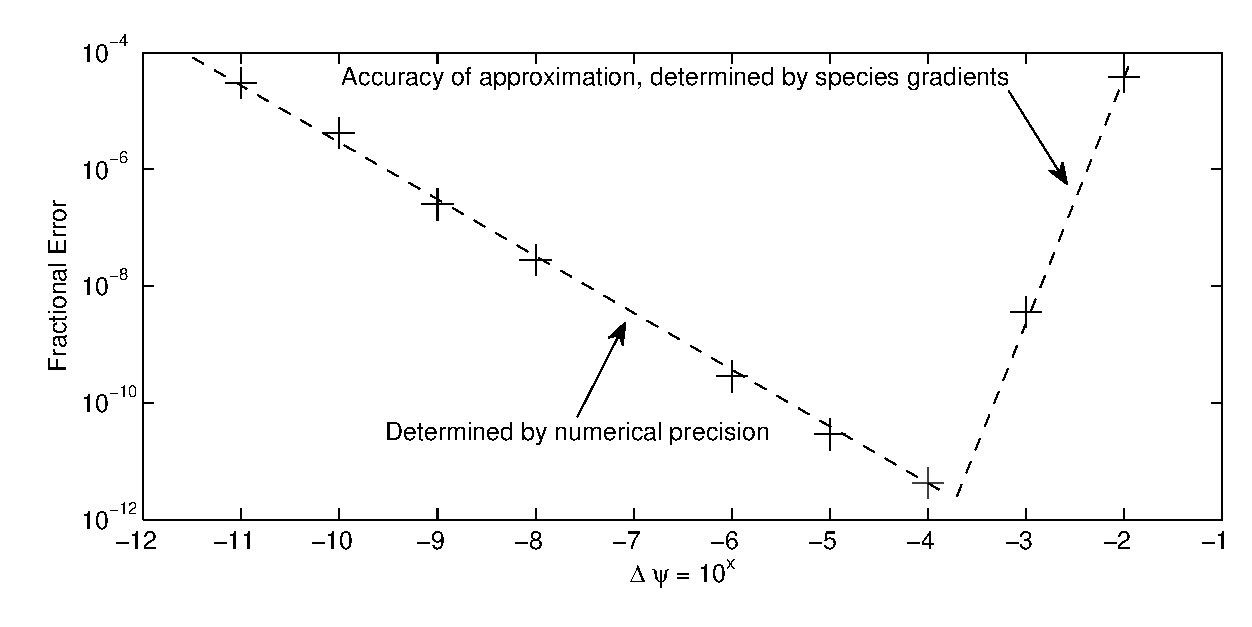
\includegraphics[width=0.6\textwidth]{cfphi-accuracy.eps}
\caption{Numerical experiment to determine optimum $\Delta \psi$ for calculating the radial derivative of the centrifugal potential $\Phi$ for the singly charged ions Waltz standard case. The experiment was conducted in double precision and the fractional error is calculated against the analytic result Eq. \ref{eq:deriv-scions}.}

\label{fig:cfphi-acc}
\end{center}
\end{figure}

In the case of a plasma of only singly charged ions, Eq. \ref{eq:cf-quasineutral} solves exactly to give
\begin{equation}
 \Phi = \underbrace{{T_e T_i \over T_e + T_i} \left({m_i \over T_i} - {m_e \over T_e}\right)}_{\name{cf_mass_weight}} \Omega^2 (R^2-R_0^2).
\label{eq:scions}
\end{equation}
with radial derivative 
\begin{equation}
 {\partial \Phi \over \partial \psi} = \underbrace{\left[{m_i {\partial T_e \over \partial \psi}- m_e {\partial T_i \over \partial \psi}\over T_e + T_i} + 
{m_e T_i - m_i T_e \over (T_e + T_i)^2}\left({\partial T_e \over \partial \psi}+{\partial T_i \over \partial \psi}\right)\right]}_{\name{cf_dtf1}}\Omega^2(R^2-R_0^2) 
+2 \Omega^2 \underbrace{\left[{m_i T_e - m_e T_i \over T_e + T_i}\right]}_{\name{cf_mass_weight}} 
\left(R {\partial R \over \partial \psi}-R_0 {\partial R_0 \over \partial \psi}\right)
\label{eq:deriv-scions}
\end{equation}
%ADD UPRIME PIECE HERE, and in COMPLETE SET OF EQUATIONS, and in solver above
If the bulk ion species is singly charged, these quantities are evaluated in the code in \name{rotation} with the labelled function provided by \name{components} to provide a check on the solution of the root finding algorithm.  

The density $n_R$ and density gradient $1/L_n=(1 / L_n)_{R_0}$ (Eq. \ref{eq:gradients}) are defined for each species at the point on the flux surface at which $R=R_0$.  Two choices for the definition of $R_0$ are available in the code, which are selected by the input variable \name{R0\_loc} in the \name{geom} namelist.  The option \texttt{R0\_loc='axis'} sets $R_0$ as the major radius of the magnetic axis (but the reference point is not on the axis itself), whilst the default \texttt{R0_loc='LFS'} sets $R_0$ to be the value of $R$ at $s=0$, in the plane of the magnetic axis at the low field side (for general geometry this may \textit{not} be equivalent to the maximum $R$).  This choice alters only the definition of the geometry quantities $\mathcal{J}$ and $\mathcal{K}$ .  In the rotating case, the effective density gradient varies over the flux surface and there is no longer one obvious definition of the density gradient as a dimensionless quantity.  For instance
\begin{equation}
{1 \over L_n^{E} } = -{1 \over n} {\partial n \over \partial \psi},\qquad
{1 \over L_n^{e1} } = -{1 \over \{ n \} } {\partial n \over \partial \psi},\qquad
{1 \over L_n^{e2} } = -{1 \over n_{R_0}} {\partial n \over \partial \psi}, \qquad
\label{eq.rlndiags}
\end{equation}
can each be argued to be a relevant quantity. The most appropriate may be determined by the nature of the particular instability being examined. These definitions can be evaluated to be

\begin{equation}
{1 \over L_n^{e} } = {\partial \cfenn \over \partial \psi} + 
\cfenn {1 \over L_T}+  {1 \over L_n} \biggr|_{R_0}, \qquad
{1 \over L_n^{e1} } = {1 \over L_n^{e} } { \exp(-\cfenn) \over
\big\{ \exp(-\cfenn) \big\} }, \qquad
{1 \over L_n^{e2} } = {1 \over L_n^{e} }  \exp(-\cfenn)
\label{eq.rlndiags2}
\end{equation}

Since the density gradient is an important parameter for determining the stability of many modes, GKW calculates ${1 / L^E_N }$ and ${1 / L^{e1}_n }$ and $n/n_{R_0}$ for each species as a function along the field, which is written to the file \File{cfdens.dat}, and as
a flux surface average and at the outboard midplane, which is written to screen during the initialisation phase of the code. ${1 / L^{e2}_n }$ can be trivially calculated from the other two.  It should be noted that whilst the input ${1 / L_n} |_{R_0}$ must always be the same for every species in order to satisfy quasi-neutrality, the effective  ${1 / L_n^E}$ can differ for each species.  For typical parameters of a deuterium plasma, the variation in effective density and gradient can be $30\%$ at $\Omega=1$, increasing rapidly for $\Omega>1$.

\section{Background \texorpdfstring{$E \times B$}{E x B} shear flow}

The sheared $E\times B$ velocity leads to a stabilisation of turbulence through the breaking up of eddy structures. 
This $E\times B$ shearing is always present for a purely toroidally rotating plasma but can, of course, also be related 
to a sheared poloidal rotation. 

%FJC: CHECK AGAIN FACTORS OF RHO* What happens if normalise as background potential?

The equilibrium $E \times B$ rotation 
\begin{equation}
{\bf v}_s(\psi)= {{\bf b} \times \nabla \bar{\Phi} \over B} 
\end{equation}
lies inside the flux surface.  The shearing rate in the normalised units is defined to be 
\begin{equation}
\gamma_{E}^N = {1 \over 2}\rho_*^2 {\partial^2 \bar{\Phi}_N \over \partial \psi^2} ,
\label{gamma-E}
\end{equation}
where the normalisation $\bar{\Phi}= \rho_* {T_{\rm ref} \over e}\bar{\Phi}_N$ is as for the
perturbed potential Eq.~(\ref{eq:phi-norm}).  The factor $1/2$ is present due to the definition of the
reference thermal velocity.  Since GKW treats the $E \times B$ shear independently from the centrifugal effects,
we use $\bar{\Phi}$ to distinguish the background potential of the shearing from the background potential of the rotating frame.
In physical units the shearing rate is
\begin{equation}
\gamma_E = {v_{\rm thref} \over R_{\rm ref}} \gamma_E^N = 
{1 \over B_{\rm ref}}{\partial^2 \bar{\Phi} \over \partial r^2} ,
%Contingent on \phi=r/R_{ref}
%True if r = R_{max}-R_{min}
\end{equation}
where $r=(R_{\rm max}-R_{\rm min})/2$.  The GKW shearing rate is assumed
radially constant and is defined as a flux function.  At the radial centre of the flux tube
$\bf{v_s}$ is chosen to be zero, with the result that there is no net flow over the domain.  In the
local limit with the approximations of the `$s-\alpha$' model geometry
the shearing rate is then equivalent to the familiar definition \cite{Hahm95,Burrell97}:
\begin{equation}
\gamma_E \approx {(RB_p)^2 \over B_t}{\partial^2 \bar{\Phi} \over \partial \Psi^2}
\approx {d v_s \over d r} .
\end{equation}
The flow velocity is normalised as $v_s^N=v_s / v_{\rm thref}$, and as before the index $N$ is dropped in what follows.
The sign convention here is opposite to Eq.~(\ref{eq:gradients}), so $\gamma_E<0$ corresponds to 
$\nabla E_0$ radially outwards.

Only the Doppler shift of the background $E \times B$ rotation is kept in the description, i.e. the
background $E\times B$ rotation is 
added as an additional convective term for the perturbed distribution (${\bf v}_s \cdot \nabla g$) in the gyrokinetic equation~(\ref{eqs:complete-set}), 
and we neglect the acceleration due to the background potential (${\bf v}_D \cdot \nabla \bar{\phi} F_M$). 
By omitting the latter term, the flow is implemented in conservative form and provides no drive to the turbulence, so that the 
stabilising effect may be studied in isolation.  If the acceleration term were kept, it would provide a Kelvin-Helmholtz drive to
the turbulence.  This drive is likely to be small compared to the parallel shear drive (which is kept in term VIII), but could be the subject of future work. 

With zero net flow across the flux tube one obtains
\begin{equation}
{\rm III.B} = -{\bf v}_s \cdot \nabla g \rightharpoonup - \rho_*^2 {\partial \bar{\Phi} \over \partial
\psi}{\mathcal E}^{\psi \zeta}{\partial g \over \partial \zeta} =
 - 2 {\gamma_E \psi}{\mathcal E}^{\psi \zeta}  {\partial g \over \partial \zeta} .
\end{equation}
Defining $\bar \gamma_E= 2 \gamma_E {\mathcal E}^{\psi \zeta} $ and taking the Fourier transform, the term can be written as a derivative in
Fourier space
\begin{equation} 
{\mathcal T}(-{\bar \gamma_E \psi}{\partial g \over \partial \zeta}) = \bar \gamma_E
k_\zeta {\partial \hat g \over \partial k_\psi} .
\end{equation}
The derivative represents a continuous advection (and shearing) in Fourier space in $k_\psi$.  

There are a number of subtleties associated with numerical evaluation of this derivative. A finite difference approximation cannot resolve the fine 
scale structure in Fourier space.  The `harmonic derivative' \cite{Waltz94,Miller94} is a full convolution over all modes and is equivalent to a
pseudo-spectral implementation using FFTs (as was used for the nonlinear term in Eq.~(\ref{eq:nl-term})).  
Although it correctly implements the $E \times B$ shearing term inside the computational domain, it does not represent a homogeneous shear 
flow because the flow profile does not satisfy the periodicity of the discrete Fourier transform; any turbulent structure passing through the radial
boundary will experience a discontinuity in the flow profile (which in the periodic domain has a sawtooth form).  
Since the local limit requires that the turbulence has no preference for the boundary, periodicity at the boundary must be preserved. 
The `shear-periodic' boundary condition \cite{Baron82,Schumann85,Gerz89} that moves with the mean flow accomplishes this for a finite 
difference representation in the radial direction, but does not naturally translate to the spectral representation.

In coordinates that move with the flow  \cite{Rogallo81,Zang88,Pumir96}, the `radial' wavenumbers become time dependent:
\begin{align}
\psi^\prime = \psi , &\qquad& \qquad \zeta^\prime=\zeta-\psi \bar \gamma_E t ,\\
k_\zeta^\prime = k_\zeta , &\qquad& \qquad  k_\psi^\prime = k_\psi - k_\zeta \bar \gamma_E t .
\end{align}
In these coordinates, the derivative in Fourier space becomes part of the time derivative.

For a gyrokinetic code, a time dependent wave vector requires the re-evaluation of the linear terms and Bessel functions at every time-step
and would be computationally prohibitive. 
By discretising the time dependence of the wavenumbers as a remapping of the solution vector between the original fixed wavevectors, 
this expensive re-evaluation can be avoided \cite{HammettAPS06}. 
Using only the fixed wavevector grid, the advection in Fourier space occurs in jumps only when the boundary periodicity is satisfied for a 
given mode. 
Explicitly, the remapping is implemented by tracking the number of times each wavevector has been remapped $i_r(k_\zeta)$, 
and (for $\bar{\gamma}_E > 0$) remapping the solution vector
\begin{equation}
\hat g (k_\psi, k_\zeta,s) \rightarrow \hat g (k_\psi-\Delta k_\psi, k_\zeta,s),
\end{equation}
 when the inequality
\begin{equation}
 {\rm Int}( k_\zeta \bar{\gamma}_E t / \delta k_\psi ) > i_r (k_\zeta),
\end{equation} 
is satisfied.  Here, ${\rm Int}$ is the function which returns the \textit{nearest} integer.
At the low $k_\psi$ limit the solution vector is discarded.  
This means that the method is non-conservative, but since the turbulence is characterised by a peaked spectrum 
(Fig.~\ref{fig:cyclone-linear}), the losses are negligible if the range of radial wavenumbers is suitably wide.  
For numerical stability, the remapping must occur at the same time for all points along the flux tube. 
As the metric tensor ${\mathcal E}^{\psi \zeta}$ is a flux function, see Eq.~(\ref{eq:efun-cst}), this condition is always satisfied for a 
constant shear rate along the field line.

The method in GKW differs from the standard spectral methods to model homogeneous shear flows in fluid turbulence of
Refs.~\cite{Rogallo81,Zang88,Pumir96}, where the wavenumbers must be recalculated and re-meshing occurs for all wavevectors 
at the same time. 
In GKW the method used is the one proposed by Hammett et al. in Ref.~\cite{HammettAPS06}.  
Here the `re-meshing' occurs continually (and at different times for each $k_\zeta$), and the wavenumbers stay on their original fixed grid.  
The accuracy of the method has been argued to be second order on average \cite{HammettAPS06} and
is able to capture the physics effects of a 
background shear flow whilst allowing the desirable features of the flux tube model to be retained.
 
Convergence of the remap method in $L_x / L_y$ should be checked (particularly by for the modes with lowest $k_\zeta$) by decreasing 
$\Delta k_\psi / k_{\zeta {\rm min}}$ (increasing $N_x$ and $p$ (IKXSPACE) whilst holding $N_{\rm mod}$ constant (defined later)).


\section{Purely toroidal sheared rotation in general geometry}

For this section only, we adopt the superscript $^L$ to represent quantities in the laboratory frame.  
All quantities without a superscript should be interpreted as being in the rotating frame (as in all other sections). 
The same coupling condition is derived by two routes to make clear the relationship between the frames.

The rotating frame is constructed \cite{PEE09} such that rigid body rotation $\Omega$ of the frame 
matches the plasma rotation $\omega_\phi^L$ on the local flux surface.  The angular rotation then transforms
as 
\begin{equation}
\omega_{\phi}(\psi)=\omega_{\phi}^L(\psi)-\Omega 
\label{eq:transform}
\end{equation}
such that $\omega_{\phi}(\psi)=0$ (and hence ${\bf
v_s}=0$) at the centre of the radial domain. 

\subsection{In comoving frame}

For a purely toroidal rotation, decomposing the toroidal flow into its parallel and perpendicular components gives
\begin{equation}
u_\parallel \mathbf{b} +  \mathbf{v_s} = s_{\rm B} R \omega_\phi(\psi) R \nabla \varphi,
\label{eq:toroidal}
\end{equation}
where $\varphi$ is the toroidal angle. Since \eq{toroidal} is written in the comoving frame,
 it reads $0+0=0$ in the centre of the flux tube.
From the normalisations above, one can show that in the normalised units
\begin{equation}
 \mathbf{v_s} = {1 \over 2} \rho_*^2 {\mathbf{b} \times \nabla \psi \over
B} {\partial \bar{\Phi} \over \partial \psi}.
\end{equation}
Taking the bi-normal component of \eq{toroidal} one finds
\begin{equation}
 u_{\parallel} \underbrace{\mathbf{b} \cdot \nabla \zeta}_{=0} +  {1 \over 2}
\rho_*^2 \underbrace{{\mathbf{b} \times \nabla \psi \over B}\cdot \nabla
	\zeta}_{=2\mathcal{E}^{\psi \zeta}}{\partial \bar{\Phi} \over \partial \psi} = s_{\rm B} R^2 \omega_{\phi}(\psi)
\underbrace{\nabla \phi \cdot \nabla \zeta}_{=-1/2\pi R^2},
\end{equation}
hence
\begin{equation}
 {1 \over 2} \rho_*^2 {\partial \bar{\Phi} \over \partial \psi} = - {s_{\rm B} \over 4 \pi}{1 \over
\mathcal{E}^{\psi \zeta}}\omega_{\phi}(\psi),
\label{eq:comoving}
\end{equation}
which upon differentiation gives the coupling relation
\begin{equation}
 \underbrace{{1 \over 2} \rho_*^2 {\partial^2 \bar{\Phi} \over \partial \psi^2}}_{\gamma_E} = - {s_{\rm B} \over 4 \pi}\left[{1 \over
\mathcal{E}^{\psi \zeta}}\underbrace{\partial \omega_{\phi} \over \partial \psi}_{\rm u^\prime} +
\underbrace{\omega_\phi}_{=0}{\partial \over \partial \psi} \left({1 \over \mathcal{E}^{\psi \zeta}}\right)\right].
\label{eq:coupling}
\end{equation}
Note that the second term on the right is zero when evaluated at the centre of the flux tube.
All quantities in the above equation are flux functions, hence the shear rate will always be a
flux function, as required for the discrete remapping method.


\subsection{Relation to lab frame}

In the laboratory frame \eq{toroidal} becomes 
\begin{equation}
u_\parallel^L \vec{b} + {\bf v}_s^L  = s_{\rm B} R \omega_\phi^L(\psi) R \nabla \varphi.
\label{eq:toroidal2}
\end{equation}
Taking the binormal component leads to
\begin{equation}
 {1 \over 2} \rho_*^2 {\partial \bar{\Phi}^L \over \partial \psi} = - {s_{\rm B} \over 4 \pi}{1 \over
\mathcal{E}^{\psi \zeta}}\omega^L_{\phi}(\psi),
\end{equation}
and taking the radial derivative gives
\begin{equation}
 {1 \over 2} \rho_*^2 {\partial^2 \bar{\Phi}^L \over \partial \psi^2} = - {s_{\rm B} \over 4 \pi}\left[{1 \over
\mathcal{E}^{\psi \zeta}}{\partial \omega^L_{\phi} \over \partial \psi} + \omega^L_{\phi}{\partial \over \partial
\psi} \left({1 \over \mathcal{E}^{\psi \zeta}}\right)\right],
\end{equation}
which has the same form as \eq{coupling} but different values.

To make explicit the relationships between the quantities, the previous equation 
is rewritten (using \eq{transform}) in terms of the rotating frame quantities.
Since the frame rotates rigidly, ${\partial \Omega \over
\partial \psi}=0$ and ${\partial \omega / \partial \psi} = {\partial \omega^L / \partial \psi} = u^\prime$. 
The tensor component $\mathcal{E}^{\psi \zeta}$ is invariant under the transformation.
The electric field transforms \cite{PEE09} as
\begin{equation}
\bar{\Phi}=\bar{\Phi}^L + s_{\rm B} s_{\rm j}{2 \over \rho_*^2}\Psi \Omega ,
\end{equation}
where $\Psi$ is the (frame independent) poloidal flux with $\nabla \Psi$ radially outward, 
and the factor of $2 / \rho_*^2$ arises from the normalisation of $\bar{\Phi}$ (see Sec. \ref{signs} for clarification of signs).  
The coupling condition can then be written as 
\begin{equation}
 \underbrace{{1 \over 2} \rho_*^2 {\partial^2 \bar{\Phi} \over \partial \psi^2}
-s_{\rm B} s_{\rm j}  {\Omega}{\partial^2 \Psi \over
\partial \psi^2}}_{\gamma_E^L} = - {s_{\rm B} \over 4 \pi}\left[{1 \over
\mathcal{E}^{\psi \zeta}}{\partial \omega_{\phi} \over \partial \psi} +
\Omega{\partial \over \partial \psi} \left({1 \over \mathcal{E}^{\psi \zeta}}\right)\right],
\end{equation}
when evaluated in the centre of the flux tube where $\omega_\psi = 0$.
Since $\Psi=f(\psi)$ only, from the relation \ref{eq:efun-flux}
% \begin{equation} 
% {\cal E}^{\psi \zeta} = \frac{s_{\rm j}}{4\pi}\frac{\partial \psi}{\partial \Psi}
% \label{eq:efun-cst}
% \end{equation}
it follows that
\begin{equation}
 {\partial \over \partial \psi} \left({1 \over \mathcal{E}^{\psi \zeta}}\right) = s_{\rm j} 4 \pi 
{\partial^2 \Psi \over \partial \psi^2},
\end{equation}
hence cancellation gives 
\begin{equation}
 \underbrace{{1 \over 2} \rho_*^2 {\partial^2 \bar{\Phi} \over \partial \psi^2}}_{=\gamma_E}
 = - {s_{\rm B} \over 4 \pi}{1 \over
\mathcal{E}^{\psi \zeta}}\underbrace{\partial \omega_{\phi} \over \partial \psi}_{=u^\prime},
\end{equation}
which is the same as \eq{coupling} when evaluated at the centre of the flux tube.  The shearing rates in the two frames are therefore related by
\begin{equation}
 \gamma_E^L = \gamma_E - s_{\rm B} s_{\rm j}{\Omega}\underbrace{{\partial^2 \bar{\Psi} \over \partial \psi^2}}_{\cal{M}},
\end{equation}
but presently only $\gamma_E$ is implemented in the code.


\section{Poloidal asymmetries induced by anisotropic minorities}

In this section, all units are dimensional, except those indicated with a superscript $N$, which denotes 
a dimensionless quantity using the GKW normalisations defined in Section \ref{sec:normalisation}.

Recent experiments have observed poloidal asymmetries in heavy impurities in the presence of ion cyclotron
resonance heating (ICRH) of a light minority ion \cite{Reinke12}.  This phenomena is believed to be due to 
the anisotropy of the heated species, which sets up an equilibrium potential. 

\subsection{Reinke model \label{sec.icrh}}

 In the rotating frame of reference, the parallel
force balance for an anisotropic species $m$ (generalisation of Eq 3 of Ref. \cite{Reinke12} with a sign correction for the second term)
is 
\begin{equation}
%\vec{b} \cdot (\nabla \cdot \vec{P} n_m e Z_m \nabla_\parallel \Phi) = 
\nabla_\parallel p_\parallel - \frac{p_\parallel - p_\perp}{B}\nabla_\parallel B + n_m Z_m e \nabla_\parallel \Phi - n_m m_m \Omega^2 R \nabla R = 0
\end{equation}  
Assuming $\nabla_\parallel T_\parallel = 0$, one finds on integration
\begin{equation}
n_m = A B^{-\eta} \exp\left(-\frac{e Z_m \Phi}{T_\parallel} + \frac{m_m \Omega^2 R^2}{2 T_\parallel}\right)
\end{equation}
where $\eta = T_\perp/T_\parallel - 1$, and $A$ is a constant of integration (with dimensions of $[n B^{\eta}]$) to be determined. 
In Ref. \cite{Reinke12}, $A = \{n\}/\{B^{-\eta}\}$, but this choice is actually 
inconsistent with the definition of the flux surface average $\{ \}$; the correct definition (when $\Omega = 0$) would actually require
\begin{equation}
A_{\rm FSA}  = \frac{\{n_m\}}{\{B^{-\eta}\exp(-{e Z_m \Phi / T_\parallel})\}}. 
\label{eq.correctnorm}
\end{equation}
Although the difference between this and the normalisation of Eq. 3 of Ref. \cite{Reinke12} is small for typical parameters, the deviation
is enough to break quasi-neutrality and so the approximate normalisation of Ref. \cite{Reinke12} is not possible
to use in a code which contains a field solver.  Furthermore, defining the constant $A$ correctly as in Eq. \ref{eq.correctnorm} 
would require repeated iterations of the root finding quasi-neutrality solver condition over the whole flux surface, 
which although possible is probably unnecessary for this problem.
Instead, to be consistent with the previous definition of $n_{R0}$ as the density at $R=R_{0}$, we must have $A = n_{R0} B_{R0}^\eta$  
and thus we have
\begin{equation}
n_m = n_{R0,m} \left(\frac{B}{B_{R0}}\right)^{-\eta} \exp\left(-\frac{e Z_m \Phi}{T_\parallel} + \frac{m_m \Omega^2 (R^2-R_0^2)}{2 T_\parallel}\right)
\end{equation}

For the minority species it is also convenient to define a generalised poloidal asymmetry energy
\begin{equation}
  {\cal E}_{\Omega,\eta} = {\cal E}_{\Omega} + T_\parallel \eta \ln({B/B_{R_0}})
  \label{eq.poloidal-energy}
\end{equation}
which in the GKW normalisations is 
\begin{equation}
  {\cal E}^N_{R,\eta} = {\cal E}^N_R + T^N_\parallel \eta \ln({B/B_{R_0}})
\end{equation}
where $T^N_\parallel = T_\parallel / T^N_R T_{\rm ref}$  (set $ = 1 $ in the approximations below).  This 
fits into the previous formalism such that 
\begin{equation}
  n_m = n_{R0} \exp(-{\cal E}_{\Omega,\eta}/T_\parallel)
\label{eq.cfen-gen}
\end{equation}
The definition of $\cfen$ is unchanged for all other species (although the value of $\Phi$ inside $\cfen$ will be).

\subsection{Bilato model \label{sec.icrh2}}
The Reinke model makes another approximation, by taking $p_\perp$ as a flux function.  The self-consistent solution worked out by Bilato \cite{Bilato14} gives a reduction in the asymmetry compared to the Reinke model roughly equivalent to transforming $\eta \rightarrow \eta^{3/4}$.  This model is also implemented in GKW, and is selected by using an input value of $\frac{T_{\perp R0}}{T_{\parallel}} < 0$, where the absolute value is used by the code.

The exact solution is 
\begin{equation}
 n_m = n_{R0,m} \frac{T_{\perp}(\theta)}{T_{\perp R0}}  \exp\left(-\frac{e Z_m \Phi}{T_\parallel} + \frac{m_m \Omega^2 R^2}{2 T_\parallel}\right)
\end{equation}
where
\begin{equation}
 \frac{T_{\perp}(\theta)}{T_{\perp R0}} = \left [ \frac{T_{\perp
 R0}}{T_{\parallel}} + \left(1 - \frac{T_{\perp R0}}{T_{\parallel}} \right )\frac{B_{R0}}{B} \right ]^{-1}.
\end{equation}
The generalised asymmetry energy for the minority is then defined such that Eq. \ref{eq.cfen-gen} still holds, with
\begin{equation}
    {\cal E}_{\Omega,\eta} = {\cal E}_{\Omega} + T_\parallel \ln({T_{\perp R0}}/{T_{\perp}(\theta)})
\label{eq.poloidal-energy2}
\end{equation}
which in the GKW normalisations is 
\begin{equation}
   {\cal E}^N_{R,\eta} = {\cal E}^N_R + T^N_\parallel \ln({T_{\perp R0}}/{T_{\perp}(\theta)})
\end{equation}
where $T^N_\parallel = T_\parallel / T^N_R T_{\rm ref}$  (set $ = 1 $ in the approximations below).

\subsection{Transformations of input parameters}

If, as is usual in GKW, we take $R_0 = R_{\rm LFS}$, then the consequence is that the minority
fraction $f_{\rm min} = \{n_m\}/\{n_e\}$ differs strongly from the value of $n_{R0,m} / n_{R0,e}$ in the presence of anisotropy.

However, in some cases, (particularly those of a strongly anistropic minority species)
it is desirable that the code density inputs can be specified in the form of flux surface averages,
because this is the canoncial conserved quantity in the absence of radial transport.  Such an input specification 
also removes the need for post-processing of the output quantities as dsecribed in \ref{sec.memo-icrh}.

For the reasons given in the preceding section, defining $n_{\rm input} = \{n\}$ and $rln_{\rm input} = R_{\rm ref}/L_{\{n\}} = 1/\{n\} \partial \{n\} / \partial \psi$
using the flux surface averaged densities requires an extra layer of iterative numerical solutions.

ITERATIVE transformation scheme under development, to be documented shortly....

\subsection{Implementation}

Using the generalised quasi-neutrality root finding solver for $Q(\Phi) = 0$ described in Sec. \ref{cfphi} above, it is then straightforward to 
insert the additional $B^{-\eta}$ dependence for a minority species.  Since GKW also requires and computes radial derivatives of $\Phi$, 
a maximum of 7 parameters are potentially required: 
\begin{equation}
( n_{\rm input,m}/n_{\rm ref},\qquad {T_\perp R0}/T_\parallel,\qquad {\partial (T_{\perp R0}/T_\parallel) / \partial \psi},\qquad
 T_\parallel,\qquad  \partial T_\parallel / \partial \psi,\qquad Z_m,\qquad m_m ).
\end{equation}
We remind the reader that $\psi = r/R_{\rm ref}$ is the dimensionless radial coordinate used in GKW.  Note that the minority mass is not required as an input in the case when $\Omega = 0$.

In addition, it can be useful to include the asymmetric potential generated by the minority species without simulating it as a separate gyrokinetic species (combination method: NOT PRESENTLY WORKING CORRECTLY).
For this purpose, although treated separately in the background quasi-neutrality solve, the minority species is after-wards combined with the bulk ion species ($i$).  
Since $Z e \Phi / T_\parallel \ll 1$ and $f_{\rm min} \ll 1$ only ever appear in combination if the exponential is expanded as series, 
the values of $T_\parallel$ and $\partial T_\parallel / \partial \psi$ make a negligible impact on the results 
(tested for $f_{\rm min} = 0.1$ and $T_\parallel/T_{\perp R0} = 10.0 $). 
For simplicity, these parameters are therefore neglected in the combination method, and where required, the code makes the assumption that $T_i = T_\parallel$.  (This assumption is required to have a value in the code, but in reality it does not affect the results). Only one mass is used for the combined species.  Since the mass does not appear in the anisotropy effect, the average mass of the minority plus bulk should be given
to model the centrifugal and kinetic effects correctly, but using the assumption $m_m = m_i$ will likely give almost identical results 
for most parameters.  Outside the quasi-neutrality solve, the two species are combined, with $n_{R0,t} = n_{R0,i} + n_{R0,m} Z_m / Z_i$ such that $n_t = n_i + n_m Z_m / Z_i $ everywhere, which gives a resulting asymmetry energy of
\begin{equation}
% Line below only when the species have the same Z
%  {\cal E}_{\Omega,\eta,t} =  {\cal E}_{\Omega,\eta,m} - \ln\left(n_{RO,i} (B/B_{\rm ref})^\eta + n_{RO,m}\right)
   {\cal E}_{\Omega,\eta,t} =  -\ln\left(n_{R_0,i}\exp(-{\cal E}_{\Omega,i}) + \frac{n_{R_0,m} Z_m}{Z_i}\exp(-{\cal E}_{\Omega,\eta,m})\right) + \ln(n_{R_0,t})
\end{equation}
such that quasi-neutrality is still satisfied everywhere for the reduced set of species.  

Because the combination option means that the asymmetry does not require an additional gyrokinetic species, the 
input parameters $n_{\rm input,m}/n_{\rm ref}, T_{\perp R0}/T_\parallel, \partial (T_{\perp R0}/T_\parallel) / \partial \psi^N, Z_{\rm min}$ are 
separated from the individual species inputs and appear in the \name{SPCGENERAL} namelist as the array \name{icrh_params(1,2,3,4)}.
respectively.  

If instead the minority is treated as a full gyrokinetic species (independent method), the species is identified with
\name{background='ICRH'} in the species namelist. This allows the fully general case without the (mild) 
assumptions on the parameters $m_m, T_\parallel$ and $\partial T_\parallel / \partial \psi^N$ required for 
the combination option.  In this case, $n_{\rm input,m}/n_{\rm ref}$ and $Z_{\rm min}$ are taken from the species inputs \name{dens} and \name{Z} respectively
(the first and last inputs \name{icrh_params(1,4)} are not used), and the species inputs \name{temp} and 
\name{rlt} describe $T_\parallel^N$. In the gyrokinetic equation, this species is then treated as a Maxwellian with temperature $T=T_\parallel$
(i.e., there is no bi-Maxwellian option implemented for $F_0$). Strictly, a more accurate approximation would be a Maxwellian with $T=(T_\parallel T_\perp^2)^{1/3}$, which might be more accurate for collisions or neoclassics.

After the solver completes, the code runs self-consistency checks on the quasi-neutrality of the gradients of the flux surface averages, which is a strong test on the consistency of the solver, using both the diagnostics in Eq. \ref{eq.rlndiags}, and the transformations described in Sec. \ref{sec.memo-icrh}.  The gradient of the flux surface average
\begin{equation}
-\frac{1}{\{n\}}\frac{\partial \{n\}}{\partial \psi} =  \left \{1/L_n^{e1}\right\}
\end{equation}
for the minority is calcuated using 
\begin{equation}
 {1 \over L_n^{e,N} } = {\partial {\cal E}_{R,\eta} \over \partial \psi} + 
{\cal E}_{R} {1 \over L^N_T}+  {1 \over L^N_n} \biggr|_{R_0}
\label{eq.rlndiag3}
\end{equation}
(note, the second term does NOT use the generalised energy $ {\cal E}_{R,\eta}$) 
with
\begin{equation}
 {1 \over L_n^{e1,N} } = {1 \over L_n^{e,N} } { \exp(-\cfenn) \over
\big\{ \exp(-\cfenn) \big\} }, \qquad
\end{equation}
which is the generalisation of Eq. \ref{eq.rlndiags2}).  The first term in Eq. \ref{eq.rlndiag3} is evaluated with the derivatives appearing in Sec. \ref{sec.memo-icrh}, 
%or Sec. \ref{sec.memo-icrh2}, 
and the results of the checks are output to screen. 

\pagebreak

\subsubsection{Examples of anisotropic minority input setup}

Since the quasi-neutrality solver is only activated for centrifugal effects, the switch \name{cf_trap=T} must also be set
even in the absence of rotation.  Here we present two example input setups for a 
$5\%$ helium-4 minority with $T_\perp/T_\parallel = 4$ and $\partial (T_\perp/T_\parallel) / \partial \psi = -8.5$.
First treating the minority species as a gyrokinetic species, (independent method) we have:
\begin{footnotesize}
\begin{verbatim}
&GRIDSIZE
number_of_species = 4
/
&SPCGENERAL
icrh_params = 999, 4.0, -8.5, 999  ! First and last not used
/
&SPECIES ! D ions
mass = 1.0000, dens = 0.90, z = 1.00, rlt = 5.5, rln = 2.5, temp = 1.0, uprim = 0.0
/
&SPECIES ! electrons
mass = 2.7e-4, dens = 1.00, z = -1.0, rlt = 4.5, rln = 2.5, temp = 1.2, uprim = 0.0
/
&SPECIES ! Molby trace impurity
mass = 48.000, dens = 0.00, z = 32.0, rlt = 6.5, rln = 1.5, temp = 1.0, uprim = 0.0
/
&SPECIES ! He ICRH minority
mass = 2.0000, dens = 0.05, z = 2.00, rlt = 9.9, rln = 2.5, temp = 2.0, uprim = 0.0
background = 'ICRH'
/
&ROTATION
cf_trap = .true.
/
\end{verbatim}
\end{footnotesize}
or, alternatively, treating the minority in combination with the bulk ions (combination method),
and giving practically identical results for $\Phi$ \texttt{and its deriviatives}: 
\begin{footnotesize}
\begin{verbatim}
&GRIDSIZE
number_of_species = 3
/
&SPCGENERAL
icrh_params = 0.05, 4.0, -8.5, 2.0  ! minority fraction, Tp/T||, d(Tperp/T||)/dpsi, Z_m
/
&SPECIES ! D ions + He minority (treated with Z = 1 in Possion and GK equations)
mass = 1.0527, dens = 1.00, z = 1.00, rlt = 5.5, rln = 2.5, temp = 1.0, uprim = 0.0
/
&SPECIES ! electrons
mass = 2.7e-4, dens = 1.00, z = -1.0, rlt = 4.5, rln = 2.5, temp = 1.2, uprim = 0.0
/
&SPECIES ! Molby trace impurity
mass = 48.000, dens = 0.00, z = 32.0, rlt = 6.5, rln = 1.5, temp = 1.0, uprim = 0.0
/
&ROTATION
cf_trap = .true.
/
\end{verbatim}
\end{footnotesize}

\subsubsection{Tests}

\begin{itemize}

\item The combination method and the independent method give identical asymmetries.
\item Quasi-neutrality is always satisfied everywhere, with all $\eta$, and all $\Omega$, all geometries, for both $R_0$ choices, 
and arbitrary non-trace species combinations.
\item Quasi-neutrality in the gradients is satisfied at all locations, and in the flux surface average density, checked using the formulae of Sec. \ref{sec.memo-icrh}.
\item The $\Phi$ asymmetry scales linearly with $f_m$, $Z_m$ and $\eta$, and is practically independent of $T_\parallel$.
\item High-Z impurity asymmetries are of the same magnitude as in Ref. \cite{Reinke12} for the given parameters.
\
%STILL TO DO:

%\item Investigate sensitivities of the radial derivatives
%\item Fix radial derivatives for combination method

\end{itemize}


% related to auctex mode and latex-preview-mode in Emacs:
%%% Local Variables:
%%% mode: latex
%%% TeX-master: "doc"
%%% End:
